\chapter{为创作者而作的教程}
\section{关于如何使用\LaTeX 编写模板}\label{sec:关于如何使用LaTeX编写模板}

\sectionAuthor{Jiaqi Z.}

% 请在下面的Abstract当中填写这一节的知识点
\begin{Abstract}
    \item 一些基本的\LaTeX 语法
    \item 如何输入公式
    \item 如何插入代码
    \item 如何插入图片
    \item 如何插入创建索引
\end{Abstract}

对于创作者而言,这一部分可以帮助你快速了解\LaTeX 的基本语法,帮助你按照规范编写正确的文件。同时对于普通读者而言,这一部分也是你了解本书内容样式的一部分。

因此,任何人都应当阅读这一部分\footnote{对于创作者而言,还应当试着从GitHub上寻找源码阅读}。

\subsection{文章结构}\label{subsec:关于如何使用LaTeX编写模板-文章结构}

请在编写正文内容时,以“节”(section)为单位创建tex文档,同时为方便引用,请在每个小节的后面按照\verb|\label{sec:节标题}|的格式创建标签。

若需要添加小节,使用\verb|\subsection{小节标题}|命令,同时类似于上方关于节标题标签的创建规范,以\verb|\label{subsec:节标题-小节标题}|的格式创建标签,方便他人引用。

对于更小一级的小节(\verb|\subsubsection{}|),对标签不作规范。事实上,我们不建议在引用时涉及到这一层级。通常涉及到小节即可。

\begin{attention}
    若你需要修改某一节(或小节)的标题,编译后需要确认是否与他人的标签产生冲突(这通常出现在他人提前按照原有格式引用后发生了修改,从而导致无法指向正确标签)。因此,你需要检查编译后文件是正确的,\emph{至少要求通过编译},在必要时需要修改他人代码当中的引用标签与新标签一致。
\end{attention}

对于正文内容,请使用正常的\LaTeX 语法。例如,当你希望对某一段文字进行强调时,请使用\verb|\emph{}|语句。例如,\emph{这是一句强调的话}在代码中体现为\verb|\emph{这是一句强调的话}|。你并不需要关注具体的强调格式--\LaTeX 会按照统一的格式进行编排。

当你希望分段时,使用空行即可。

对于条目,请在必要的时候使用\verb|itemize|环境(没有顺序列表)或\verb|enumerate|环境(有顺序列表)。在环境内使用\verb|\item|进行编号。环境之间可以嵌套。例如:

\begin{itemize}
    \item 列表1
    \item 列表2
    \begin{enumerate}
        \item 列表2-1
        \item 列表2-2
    \end{enumerate}
    \item 列表3
\end{itemize}

在代码中体现为:

\begin{lstlisting}[frame=line]
\begin{itemize}
    \item 列表1
    \item 列表2
    \begin{enumerate}
        \item 列表2-1
        \item 列表2-2
    \end{enumerate}
    \item 列表3
\end{itemize}
\end{lstlisting}

大多数用法与基本\LaTeX 一样,少有的需要特别注意的是波浪线符号\texttilde,如果使用习惯的打法\verb|\~|则会显示较小,因此,在输入时请使用修改后的波浪线符号\verb|\texttilde|,或者使用更简洁的形式\verb|\ttilde|。例如,在使用\verb|\~/bin|显示的结果为\code{\~/bin}而使用\verb|\ttilde/bin|显示为\code{\ttilde/bin}

\subsection{一些特殊的格式}\label{subsec:关于如何使用LaTeX编写模板-一些特殊的格式}

在有些时候,会希望在书后添加一些辅助性的文字说明,可以使用\emph{脚注}。脚注应当使用命令\verb|\footnote{}|创建,例如,

\begin{lstlisting}[frame=line]
这里有一段文字\footnote{这里是说明性的脚注}。
\end{lstlisting}

编译后效果为

这里有一段文字\footnote{这里是说明性的脚注}。

此外,为了激发读者思考,在编写时可以添加一些简单的思考题贯穿于正文中。这些思考题不应当很难(对于较难的题目,可以放置在一节后),应当做到读者经过简单的思考(约1分钟以内)即可得到正确答案。此时在编写时应当将答案放置在题目后面,考虑到避免读者直接看到答案,所有答案都按照特定的格式排版。在编写时应当使用\verb|\answer{}|命令,例如:

\begin{lstlisting}[frame=line]
这里是思考题。

\answer{倒着看便是答案}
\end{lstlisting}

排版的效果是

这里是思考题。

\answer{倒着看便是答案}

\subsection{一些特殊的环境}\label{subsec:关于如何使用LaTeX编写模板-一些特殊的环境}

为统一教程格式,当你希望添加一段让读者注意的文字时,请使用环境\verb|attention|例如,下面的语句

\begin{lstlisting}[frame=line]
\begin{attention}
    当你写注意语句时,不需要在前面加任何符号。
\end{attention}
\end{lstlisting}
在编译后的结果为:

\begin{attention}
    当你写注意语句时,不需要在前面加任何符号。
\end{attention}

类似地,对于一些补充性质的内容,可以使用\verb|extend|环境,例如:
\begin{lstlisting}[frame=line]
    \begin{extend}
        这是一段补充的内容,同样不需要在前面加任何符号。
    \end{extend}
\end{lstlisting}

编译后的结果为:

\begin{extend}
    这是一段补充的内容,同样不需要在前面加任何符号。
\end{extend}

\subsection{数学公式}\label{subsec:关于如何使用LaTeX编写模板-数学公式}

当你希望添加数学公式时,请使用\verb|equation|环境。同时,在使用\verb|\label|语句进行标签注明时,请如同代码所示那样,添加“节标题”避免冲突且方便引用。

\begin{lstlisting}[frame=line]
\begin{equation}
    \label{eqn:关于如何使用LaTeX编写模板-1}
    a^2+b^2=c^2
\end{equation}
\end{lstlisting}

\begin{equation}
    \label{eqn:关于如何使用LaTeX编写模板-1}
    a^2+b^2=c^2
\end{equation}

在引用公式时,请使用如\verb|\ref{eqn:数学公式-1}|方式进行交叉引用。\emph{请勿直接在正文内写编号}以免出现引用错误。

\begin{attention}
    在引用公式时,所引用的公式尽量保持在本节内。同时,为避免他人引用,请在编写完成后尽量不要修改相关标签。

    为避免公式删除导致的错误,如确实需要引用其他章节的公式,一个较合理的做法是将其他章节的公式在使用时拷贝至当前章节,同时另起标签名。之后的引用限制在当前章节内。
\end{attention}

如需要添加多行公式,请使用\verb|gather|环境或\verb|align|环境。例如,

\begin{lstlisting}[frame=line]
\begin{gather}
    a^2+b^2=c^2\label{eqn:关于如何使用LaTeX编写模板-2}\\
    \int_a^bf(x)\dd{x}=F(b)-F(a)\label{eqn:关于如何使用LaTeX编写模板-3}
\end{gather}
\end{lstlisting}

\begin{gather}
    a^2+b^2=c^2\label{eqn:关于如何使用LaTeX编写模板-2}\\
    \int_a^bf(x)\dd{x}=F(b)-F(a)\label{eqn:关于如何使用LaTeX编写模板-3}
\end{gather}

\subsection{图片}\label{subsec:关于如何使用LaTeX编写模板-图片}

当添加图片前,请首先在相关文件夹内创建名为\verb|fig|的文件夹,在插入图片时如正常\LaTeX 代码插入即可。同样,在添加标签时,使用节标题作为开头方便他人引用。即使用下面的代码方式

\begin{lstlisting}[frame=line]
\begin{figure}
    \centering
    \includegraphics[width=1\linewidth]{图片路径}
    \caption{图片标题}
    \label{fig:关于如何使用LaTeX编写模板-标签}
\end{figure}
\end{lstlisting}

\begin{figure}
    \centering
    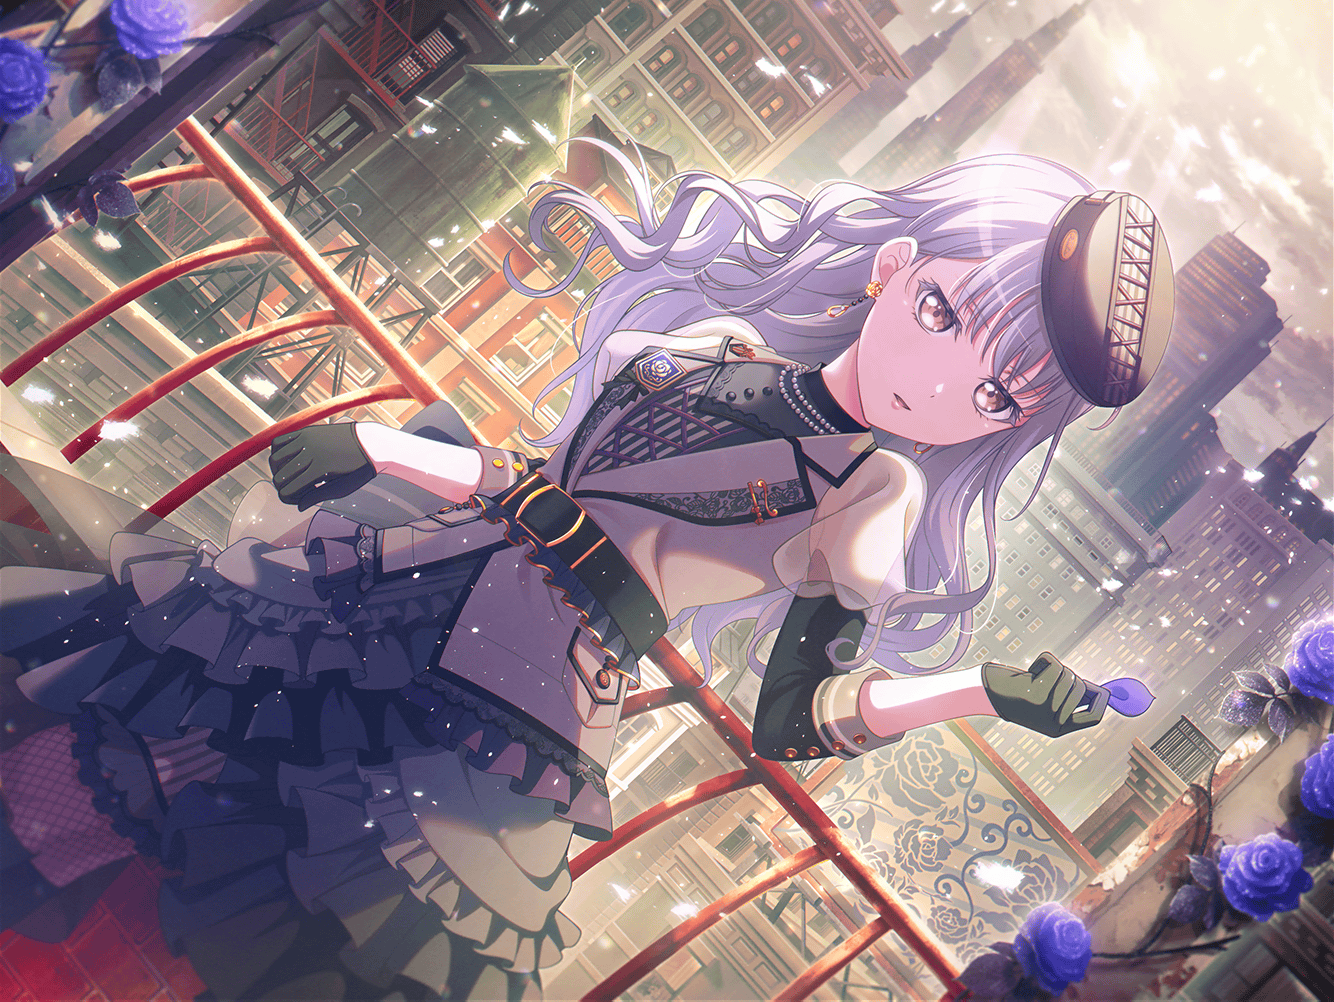
\includegraphics[width=1\linewidth]{fig.png}
    \caption{图片标题}
    \label{fig:关于如何使用LaTeX编写模板-标签}
\end{figure}

\begin{attention}
    在引用图片时,务必使用\verb|\ref{fig:节标题-标签}|进行引用。例如,图\ref{fig:关于如何使用LaTeX编写模板-标签}。不要使用“如上图”、“如下图”的表述形式,以免图片位置发生移动造成指代不明。
\end{attention}

\subsection{代码}\label{subsec:关于如何使用LaTeX编写模板-代码}

代码使用\verb|lstlisting|环境。

\begin{lstlisting}
SYSTEM = O
ISMEAR = 0
SIGMA = 0.05
NSW = 1
\end{lstlisting}

如果希望在代码左侧添加行号以示说明,请在引用环境的右侧添加\verb|numbers=left|设置,即采用下面的代码:

\begin{lstlisting}[frame=line]
\begin{lstlisting}[numbers=left]
    ..
\end{lstlisting}

得到效果如下所示

\begin{lstlisting}[numbers=left]
SYSTEM = O
ISMEAR = 0
SIGMA = 0.05
NSW = 1
\end{lstlisting}

\begin{attention}
    若你希望在代码块中添加代码名称(例如文件名),可以使用\verb|caption|选项进行说明,例如,下面的代码:
    \begin{lstlisting}[frame=line]
\begin{lstlisting}[caption=简单的INCAR文件]
    ..        
    \end{lstlisting}

    实际编译后结果为
    \begin{lstlisting}[caption=简单的INCAR文件]
SYSTEM = O
ISMEAR = 0
SIGMA = 0.05
NSW = 1
    \end{lstlisting}

\end{attention}

\subsection{添加索引}\label{subsec:关于如何使用LaTeX编写模板-添加索引}

建议在编写过程中,为文中的程序关键字创建索引。为方便使用,可以使用命令\verb|\keyword{}|。例如,在VASP讲解SIGMA函数时,可以使用下面的代码

\begin{lstlisting}[frame=line]
\keyword{SIGMA}
\end{lstlisting}

从而在表述关键字的同时创建索引。同时,也可以使用\verb|\keywordin{}{}|的形式创建带有所属关系的索引,例如

\begin{lstlisting}[frame=line]
\keywordin{INCAR}{SIGMA}
\end{lstlisting}

便是创建了属于\code{INCAR}条目下的\code{SIGMA}索引。

\begin{attention}
    在编写时,鼓励使用索引方便他人根据关键字直接检索。在创建索引时,请提前确认现有的索引表是否有现成的索引。例如,\\\verb|\keyword{SIGMA}|和\verb|\keywordin{INCAR}{SIGMA}|会得到不同的结果。

    同时,在编写过程中已经将输出和索引集成在一个命令中,你不需要特地再编写一个输出的命令如\code{SIGMA$\backslash$keyword\{SIGMA\}},只需要使用\\\code{$\backslash$keyword\{SIGMA\}}便可在输出\code{SIGMA}的同时创建索引。
\end{attention}

对于一些特殊的内容,可能不希望给出索引(通常是命令或者文件名等),它们既不属于关键字,也不属于简单的英文单词。为了将它们区分,使用\verb|\code{}|命令进行编写。例如,\verb|\code{cd \$OLDPWD}|的输出结果为\code{cd \$OLDPWD}

\begin{attention}
    在一些特殊的情况下(例如上面的例子),可能会包含\LaTeX 本身的特殊符号(如\$本身作为公式符号)。在输入时,应当使用反斜杠$\backslash$ 作为转义字符。
\end{attention}
